\documentclass[UTF8]{ctexart}
\usepackage{amsmath}
\usepackage{amssymb}
\usepackage{booktabs}
\usepackage{background}
\usepackage{caption,subcaption}
\usepackage{CJKfntef}
\usepackage{cprotect}
\usepackage{enumitem}
\usepackage{fancyhdr}
\usepackage{float}
\usepackage{fontspec}
%\usepackage{fourier}
\usepackage{geometry}
\usepackage{listings}
\usepackage{makecell}
\usepackage{tikz}
\usepackage{url}
\usetikzlibrary{arrows.meta}
\usepackage{xcolor}

\geometry{a5paper, top=0.1cm, left=1cm, right=1cm, bottom=1cm, footskip=0.1cm}
\setCJKmainfont[BoldFont={汉仪文黑-85W},ItalicFont={方正苏新诗柳楷简体}]{汉仪文黑-55W}
\setfontfamily\Issue{Century Schoolbook}
\setfontfamily\Genshin{Genshin Teyvat Lingua Franca}
\newCJKfontfamily\TitleFont{思源宋体 CN Heavy}
\newfontfamily\timesnewroman{Times New Roman}
%\reversemarginpar

\pagestyle{fancy}
\fancyhf{}
\cfoot{\sffamily\footnotesize{-\ \thepage\ -}}
\CTEXsetup[format={\bfseries\large}]{paragraph}
%\CTEXsetup[format = {\centering\bfseries\large}, beforeskip = 3pt, afterskip = 3pt]{section}

\colorlet{darkcyan}{cyan!50!black}
\newcommand\Black[1]{\textcolor[gray]{0.3}{#1}}
\newcommand\Brown[1]{\textcolor[HTML]{998A4E}{#1}}
\newcommand\Emph[1]{\colorbox{green!10}{\textcolor{green!30!black}{#1}}}
\newcommand\Notes[1]{\textcolor{yellow!50!black}{\small #1}}
\newcommand\Example[1]{\textcolor{cyan!70!black}{\small #1}}

\renewcommand\d{\mathrm{d}}

\lstset{
    basicstyle=\small\ttfamily, %注意行末有逗号!
    keywordstyle=\bfseries\color{blue!70!black},
    commentstyle=\color{cyan!90!black},
    stringstyle=\color{green!40!black},
    columns=flexible,
    numbers=left,
    numberstyle=\footnotesize,
    escapechar=`,
    frame=shadowbox,
    %rulesepcolor=\color{red!20!blue!20!green!20}
    backgroundcolor=\color{cyan!5!white},
    language=C,
    tabsize = 4,
    breaklines = true,
}

\newcommand\IssueNumber{49}
\newcommand\Date{2025-3-2}
%\newcommand\Contributer{@金光日}
\newcommand\Subject{C++ 编程}


\begin{document}
\backgroundsetup{contents=
\includegraphics{上半示例.png}, center, scale=1, angle=0, opacity=1}
\BgThispage
\begin{center}
%{\scriptsize\Issue \textcolor[HTML]{C8BA83}{\Genshin WEEKLY TIPS}}
\phantom{...}

{\Large\textcolor{brown!40!white}{\makebox[10cm][s]{\Genshin WEEKLY KNOWLEDGE TIPS}}}

\vspace{-2em}

{\Huge\bfseries\TitleFont \Black{知\ 识\ 小\ 料}}


\vspace{-0.1cm}
{\footnotesize \Brown{「电计 2203 班」周常规知识整理共享}}
\end{center}

\vspace{-0.5cm}


\begin{figure}[H]
\hspace{1cm}
\begin{minipage}[t]{0.3\textwidth}
\centering
    \Brown{\Genshin ISSUE}

    \vspace{-0.6cm}
    \Huge \Issue\slshape\bfseries\Black{\IssueNumber}
\end{minipage}
\hfill
\begin{minipage}[t]{0.35\textwidth}
\centering
    \Brown{日期:\Date} \\
%\vspace{-0.1cm}
%    \Brown{贡献者:\Contributer} \\
\vspace{-0.1cm}
    \Brown{学科:\Subject} \\
\end{minipage}
\hspace{0.8cm}
\end{figure}

{\color{cyan!50!black}
\begin{center}
    C++ STL 总结(下)
\end{center}

STL 是一个功能非常强大的容器库,有许多内置的数据结构与算法实现。承袭「知识小料」·其三十,本期给出了映射表 \verb!map!、集合 \verb!set! 与多重集 \verb!multiset!、字符串 \verb!string! 的使用方法。
}

提醒:参加 CSP 认证考试的同学可以将「知识小料」·其三十和本期「知识小料」打印到纸上,以作为参考资料带入考场。

现安利一个「万能头文件」:\cprotect\Emph{\verb!#include<bits/stdc++.h>!},这个头文件可以代替以下所有容器库的头文件。

\section{映射表:map}
头文件:\verb!#include<map>!

map 容器是一个键值对的映射,其内部以红黑树实现,查找效率高。其基本声明方法 \verb!map<key_type, val_type> name;! 表示建立 \verb!key_type! 到 \verb!val_type! 的映射。

声明举例:
\begin{lstlisting}[numbers=none]
map <string, int> hash; //从字符串到整数的映射
map <long long, bool> vis; //从长整型到布尔型的映射
map <pair<int,int>, int> count; //从二元组到整型的映射
\end{lstlisting}

\paragraph{基本操作} 有 size、empty、clear、begin、end 操作,分别表示元素个数、是否为空、清空、首迭代器、尾迭代器。

假设 $h$ 是一个映射,对 $h$ 的基本操作如下:
\begin{table}[H]
    \centering
    \begin{tabular}{ll}
        \verb!h.size()! & 返回 $h$ 的元素个数  \\
        \verb!h.empty()! & 返回 $h$ 是否为空的指示,为空时返回 1,否则为 0 \\
        \verb!h.clear();! & 清空 $h$ 的所有元素 \\
        \verb!h.begin()! & 返回 $h$ 的首迭代器  \\
        \verb!h.end()! & 返回 $h$ 的尾迭代器  \\
    \end{tabular}
\end{table}

\paragraph{[] 操作符}
\verb!h[key]! 返回 key 所映射到的 value 值,也就是将 key 直接作为下标进行查询。内部时间复杂度为 $O(\log n)$。这是 map 容器广受欢迎的一个用法。

我们可以读 \verb!h[key]! 的值,也可以对 \verb!h[key]! 写入新值。例如,假定建立了一个字符串型到整型的映射(\verb!map <string,int> h!),那么可以用形如 \verb!h["DUT"]! 的语句获得字符串 \verb!"DUT"! 对应的整数——整数含义由用户自行规定(如字符串出现的次数),也可以用形如 \verb!h["DUT"]=3! 的语句改变映射值。

{\color{gray}\small 此外,若要查找的 key 不存在,则执行 \verb!h[key]! 后,会在内存空间中创建一个结果二元组 \verb!(key,zero)!,返回 zero 的引用。其中的 zero 代表广义零值,如数字 0、空字符串等。如果查找后不对 \verb!h[key]! 赋值,则 $h$ 可能会包含许多无用的零值二元组。因此,可以先使用 \verb!find! 方法检查 key 的存在性后,再使用 [] 操作符查询。}

\backgroundsetup{contents=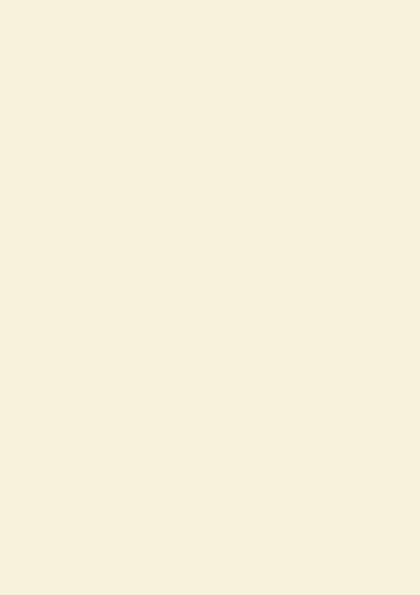
\includegraphics{空白示例.png}, center, scale=1, angle=0, opacity=1}
\BgThispage

\paragraph{find 操作}
\verb!h.find(x)! 在变量名为 $h$ 的 map 中查找 key 为 $x$ 的二元组,并返回指向该二元组的迭代器。如不存在,则返回尾迭代器 \verb!h.end()!。内部时间复杂度为 $O(\log n)$。

\paragraph{insert/erase 操作}
\begin{itemize}
    \item \verb!h.insert(make_pair(key, value))! 在变量名为 $h$ 的 map 中插入一条从 key 到 value 的记录。其中 \verb!make_pair! 是一个函数名。

    \item \verb!h.erase(make_pair(key, value))! 在变量名为 $h$ 的 map 中删除一条从 key 到 value 的记录。

    \item \verb!h.erase(it)! 在变量名为 $h$ 的 map 中删除迭代器 $it$ 指向的记录。其中 $it$ 是一个定义好的迭代器。
\end{itemize}

\paragraph{map 的迭代器} 迭代器类型为 \verb!map<key_type, val_type>::iterator!,声明一个迭代器用以下方法:
\begin{lstlisting}[numbers=none]
map <key_type, val_type>::iterator it;
map <key_type, val_type>::iterator it = h.begin();
map <key_type, val_type>::iterator it = h.end();
\end{lstlisting}
迭代器的用法参见「知识小料」·其三十的 vector 的用法。

\paragraph{实例} 用 map 统计字符串出现的次数。给定 $n$ 个字符串,$m$ 个问题,每个问题询问一个字符串出现的次数。以下用字符串到整数的映射 $h$ 来记录字符串出现的次数。
\begin{lstlisting}
#include<bits/stdc++.h>
using namespace std;
int main(){
	map<string, int> h; //声明从字符串到整数的映射
	char str[101];
	int n = 5, m = 4;
	for(int i=1; i<=n; i++){
		scanf("%s",str);
		h[str]++; //键str对应的值h[str]自增1
	}
	for(int i=1; i<=m; i++){
		scanf("%s",str);
		if(h.find(str) == h.end()) printf("0\n"); //未找到字符串
		else printf("%d\n", h[str]); //找到字符串,输出str的出现次数
	}
	return 0;
}
\end{lstlisting}


\section{集合 set 与多重集 multiset}
头文件:\verb!include<set>!

这个头文件包含了有序集合 set 和有序多重集 multiset 两个容器。顾名思义,set 的元素不能重复,而 multiset 可包含多个相同的元素。这两个容器的内部也以红黑树实现,查找效率高。

声明举例:
\begin{lstlisting}[numbers=none]
set <int> s;  //整数集合
set <string> s; //字符串集合
struct rec{...}; set <rec> s; //结构体集合
multiset <int> s; //整数多重集
\end{lstlisting}

\paragraph{基本操作} 有 size、empty、clear 操作,分别表示元素个数、是否为空、清空。用法与 vector 和 map 的类似,不再赘述。

\paragraph{insert 操作} \verb!s.insert(x)! 把一个元素 $x$ 插入到集合 $s$ 中,内部时间复杂度为 $O(\log n)$。

在 set 中,若 $x$ 已存在,则执行这段代码没有效果;而在 multiset 中,无论 $x$ 是否存在都会插入一个元素。

{\color{gray}\small 事实上,set 和 multiset 中的元素会默认以从小到大方式排列,因此按照迭代器顺序可以有序地输出这些元素。}

\paragraph{erase 操作}
\begin{itemize}
    \item \verb!s.erase(x)! 从 $s$ 中删除\Emph{所有}等于 $x$ 的元素。内部时间复杂度 $O(\log n)$。
    \item \verb!s.erase(it)! 从 $s$ 中删除迭代器 $it$ 指向的元素,其中 $it$ 是一个定义好的迭代器。内部时间复杂度 $O(k+\log n)$,其中 $k$ 为所删除元素的个数。
    \item 如果想从 multiset 中删除至多一个等于 $x$ 的元素,可以利用迭代器实现:
\end{itemize}
\begin{lstlisting}[numbers=none]
multiset<data_type>::iterator it;
if((it = s.find(x)) != s.end()) s.erase(it);
\end{lstlisting}

\paragraph{find 操作}
\verb!s.find(x)! 在集合 $s$ 中查找等于 $x$ 的元素,并返回指向该元素的迭代器;若不存在,则返回尾迭代器 \verb!s.end()!。内部时间复杂度 $O(\log n)$。

\paragraph{count 操作}
\verb!s.count(x)! 在集合 $s$ 中查找等于 $x$ 的元素个数。内部时间复杂度 $O(k+\log n)$,其中 $k$ 为元素个数。

\paragraph{二分查找}
\begin{itemize}[itemsep=0pt,parsep=0pt]
    \item \verb!s.lower_bound(x)! 在集合 $s$ 中查找 $\geqslant x$ 的元素中最小的一个。
    \item \verb!s.upper_bound(x)! 在集合 $s$ 中查找 $> x$ 的元素中最小的一个。
    \item \verb!--s.lower_bound(x)! 在集合 $s$ 中查找 $< x$ 的元素中最大的一个。
    \item \verb!--s.upper_bound(x)! 在集合 $s$ 中查找 $\leqslant x$ 的元素中最大的一个。
\end{itemize}
返回的都是指向该元素的\Emph{迭代器}。内部时间复杂度 $O(\log n)$。这是集合容器广受欢迎的一个用法。

此外,对迭代器用星号引用可以返回相应的元素值,比如 \verb!*s.lower_bound(x)! 可以求得集合中 $\geqslant x$ 的元素中最小的一个的值。

\paragraph{集合的迭代器}
迭代器类型为 \verb!set(或multiset) <data_type>::iterator!。集合的迭代器支持 \verb!++! 和 \verb!--! 两个与算术相关的操作。当执行 \verb!it++! 后,迭代器 $it$ 将指向排名靠后一位的元素;当执行 \verb!it--! 后,迭代器 $it$ 将指向排名靠前一位的元素。这两个操作的内部时间复杂度为 $O(\log n)$。此外,执行 \verb!*it! 可以得到迭代器 $it$ 指向的元素。

此外:执行 \verb!++! 和 \verb!--! 操作前请检查越界,切忌超出 \verb!s.begin()! 和 \verb!s.end()! 之间的范围。

\paragraph{实例} 以下的实例中,展示了集合的插入、删除、二分查找、计数功能。
\begin{lstlisting}
#include<bits/stdc++.h>
using namespace std;
int main(){
	multiset<int> s; //多重集
	s.insert(1); s.insert(2); s.insert(5); s.insert(5); s.insert(3);
	s.insert(6); s.insert(8); s.insert(10); //s={1,2,3,5,5,6,8,10}
	cout << *s.lower_bound(5) << endl; //`\textcolor{cyan}{$\geqslant 5$}`的数中的最小者
	cout << *s.upper_bound(5) << endl; //`\textcolor{cyan}{$>5$}`的数中的最小者
	cout << *(--s.lower_bound(5)) << endl; //`\textcolor{cyan}{$<5$}`的数中的最大者
	cout << *(--s.upper_bound(5)) << endl; //`\textcolor{cyan}{$\leqslant 5$}`的数中的最大者
	cout << s.count(5) << endl; //返回5的数量:2
	// ----------------
	multiset<int>::iterator it = s.find(5); //建立一个指向元素 5 的迭代器
	if(it != s.end()) s.erase(it); //删除一个5,变成 s={1,2,3,5,6,8,10}
	cout << s.count(5) << endl; //返回5的数量:1
}
\end{lstlisting}

\section{字符串:string}
头文件:\verb!#include<string>!

字符串的使用方法如表 \ref{tab:string常用功能列表} 所示。提供一个实例,\textcolor{blue}{顺次执行}代码,表中列出结果。

\begin{table}[p]
    \centering
    \small
    \caption{string常用功能列表及实例}\label{tab:string常用功能列表}
    \begin{tabular}{ll}
    \toprule
        \textbf{代码} & \textbf{功能} \\
    \midrule
        \verb!cin>>s;! & 输入字符串,遇到空格或回车停止\\
        \verb!getline(cin,s);! & 输入字符串,保留空格 \\
        \verb!cout<<s;! & 输出字符串 \\
        \verb!s.assign(<字符串>);! & 将 s 赋值为\verb!<字符串>! \\
        \verb!s.size()! 或 \verb!s.length()! & 查询字符个数(不含结束符) \\
        \verb!s[0]!、\verb!s[1]!、…… & 查询某个字符 \\
        \verb!s1>s2! & 若 s1 字典序比 s2 大,则返回 true \\
        \verb!s.insert(<初位置>,<字符串>);! & 在 s 的\verb!<初位置>!之前插入\verb!<字符串>! \\
        \verb!s.erase(<初位置>,<字符数>);! & 从 s 的\verb!<初位置>!开始,删除\verb!<字符数>!个字符 \\
        \verb!s.append(<字符串>);! & 将\verb!<字符串>!追加到 s 的尾部 \\
        \verb!s.find(<字符串>);! & 查找\verb!<字符串>!在 s 内第一次出现的位置 \\
        \verb!s.rfind(<字符串>);! & 查找\verb!<字符串>!在 s 内最后一次出现的位置 \\
        \verb!string::npos! & 表示找不到的一种返回值 \\
        \verb!reverse(s.begin(), s.end());! & 反转整个字符串 s(这是 algorithm 头文件的函数)\\
        \verb!s.substr(<初位置>,<字符数>)! & 从 s 的\verb!<初位置>!开始,提取\verb!<字符数>!个字符作子串返回 \\
    \bottomrule
    \end{tabular}
    \begin{tabular}{lll}
    \toprule
        \textbf{行为} & \textbf{代码} & \textbf{结果} \\
    \midrule
        定义 & \verb!string s1="abcdefg";! & s1:\verb!abcdefg! \\
        定义 & \verb!string s2("hijklmn");! & s2:\verb!hijklmn! \\
        赋值 & \verb!s1.assign("abcdef");! & s1:\verb!abcdef!;s2:\verb!hijklmn! \\
        长度 & \verb!cout<<s1.size();! & 输出:\verb!6! \\
        判空 & \verb!cout<<s2.empty();! & 输出:\verb!0! \\
        随机访问 & \verb!cout<<s1[0]<<s1[2];! & 输出:\verb!ac! \\
        比较 & \verb!cout<<(s1>s2 ? "s1字典序大" : "s1字典序小");! & 输出:\verb!s1字典序小! \\
        比较 & \verb!cout<<(s1==s2);! & 输出:\verb!0! \\
        比较 & \verb|cout<<(s1!=s2);| & 输出:\verb!1! \\
        插入 & \verb!s1.insert(2,"xx");! & s1:\verb!abxxcdef! \\
        删除 & \verb!s2.erase(3,3);! & s2:\verb!hijn! \\
        后插 & \verb!s2.append("opq");! & s2:\verb!hijnopq! \\
        查找 & \verb!cout<<s1.find("x");! &  输出:\verb!2! \\
        查找 & \verb!cout<<s1.rfind("x");! & 输出:\verb!3! \\
        查找 & \verb!cout<<((s1.find("y")==string::npos) ? 1 : 0 );! & 输出:\verb!1! \\
        赋值 & \verb!s1.assign("gfedcba");! & s1:\verb!gfedcba! \\
        反转 & \verb!reverse(s1.begin(), s1.end());! & s1:\verb!abcdefg!\\
        提取子串 & \verb!cout<<s1.substr(2,4);! & 输出:\verb!cdef! \\
    \bottomrule
    \end{tabular}
\end{table}

\section{序列操作:algorithm}
头文件:\verb!#include<algorithm>!

\paragraph{排序:sort} 内部时间复杂度 $O(n\log n)$。详见「知识小料」·其三十。
\begin{itemize}
    \item 对下标为 $1\sim n$ 的数组 $a$ 排序:\verb!sort(a+1, a+1+n);!
    \item 对 vector 排序:\verb!sort(a.begin(), a.end());!
\end{itemize}

\paragraph{翻转:reverse}
\begin{itemize}
    \item 对下标为 $1\sim n$ 的数组 $a$ 翻转:\verb!reverse(a+1, a+1+n);!
    \item 对 vector 翻转:\verb!reverse(a.begin(), a.end());!
\end{itemize}

\paragraph{随机打乱:random\_shuffle} 用法与 \verb!reverse! 相同。

\paragraph{去重:unique}
\begin{itemize}
    \item 对下标为 $1\sim n$ 的数组 $a$ 去除重复元素:\verb!m = unique(a+1, a+1+n) - (a+1);!(返回值 $m$ 为去重后的元素个数,下同)
    \item 对 vector 去除重复元素:\verb!m = unique(a.begin(), a.end()) - a.begin();!
\end{itemize}

\paragraph{下一排列:next\_permutation}
将两个迭代器/指针所在闭区间指定的部分视为一个排列,\verb!next_permutation! 函数给出字典序的下一个排列。若不存在字典序更靠后的排列,返回 false;否则返回 true。

例如:排列 $\{1,2,3,4\}$ 的下一个排列是 $\{1,2,4,3\},\{1,3,2,4\},\{1,3,4,2\},\cdots$ 且当排列为 $\{4,3,2,1\}$ 时,使用该函数则返回 false,否则其他情况均返回 true。

输出所有 $n!$ 个全排列:
\begin{lstlisting}
int a[10], n=4;
for(int i=1; i<=n; i++) a[i]=i;
do{
	for(int i=1; i<=n; i++) printf("%d ",a[i]);
	printf("\n");
}
while(next_permutation(a+1, a+1+n));
\end{lstlisting}

\paragraph{上一排列:prev\_permutation} 用法与 \verb!next_permutation! 类似。

\paragraph{二分查找}
在对数组排序以后,可以使用 \verb!lower_bound! 和 \verb!upper_bound! 函数进行二分查找。对下标为 $1\sim n$ 的数组 $a$ 二分查找某个元素,用法如下:
\begin{itemize}[itemsep=0pt,parsep=0pt]
    \item \verb!*lower_bound(a+1, a+1+n, x)! 查找 $\geqslant x$ 的元素中最小的一个。
    \item \verb!*upper_bound(a+1, a+1+n, x)! 查找 $> x$ 的元素中最小的一个。
    \item \verb!*(lower_bound(a+1, a+1+n, x) - 1)! 查找 $< x$ 的元素中最大的一个。
    \item \verb!*(upper_bound(a+1, a+1+n, x) - 1)! 查找 $\leqslant x$ 的元素中最大的一个。
\end{itemize}
由于用了星号解除引用(取指针的值),因此返回的是相应的元素。\textcolor{gray}{此外,查找 $<x$ 和 $\leqslant x$ 的语句的偏移量用 \texttt{-1},而不是 set 中的 \texttt{--}。}注意:在二分查找前,请确保你的数组是\Emph{升序排列完成}的。

可以对 vector 二分查找,如 \verb!*(lower_bound(a.begin(), a.end(), x)-1)! 查找整型变长数组 $a$ 中 $<x$ 的元素中最大的一个,返回相应元素。同理,在二分查找前,请确保你的 vector 是\Emph{升序排列完成}的。

\begin{table}[htb]
    \centering
    \begin{tabular}{cc}
    \toprule
        \multicolumn{2}{c}{$a=\{1,2,3,5,5,6\}$,$n=6$} \\
    \midrule
        \verb!*lower_bound(a+1, a+1+n, 5)! & $=5$ \\
        \verb!*upper_bound(a+1, a+1+n, 5)! & $=6$ \\
        \verb!*(lower_bound(a+1, a+1+n, 5)-1)! & $=3$ \\
        \verb!*(upper_bound(a+1, a+1+n, 5)-1)! & $=5$ \\
    \bottomrule
    \end{tabular}
\end{table}


\newpage
\section{实例:2024年3月CCF-CSP第二题·相似度计算}
{\small
链接:\url{https://sim.csp.thusaac.com/contest/33/problem/1}

时间限制:1.0s;空间限制:512MiB。

\paragraph{题目背景}
两个集合的 Jaccard 相似度定义为:
\begin{equation*}
    sim(A,B) = \dfrac{|A\cap B|}{|A\cup B|}
\end{equation*}
即交集的大小除以并集的大小。当集合 $A$ 和 $B$ 完全相同时,$sim(A,B)=1$ 取得最大值;当二者交集为空时,$Sim(A,B)=0$ 取得最小值。

\paragraph{题目描述}
除了进行简单的词频统计,小 P 还希望使用 Jaccard 相似度来评估两篇文章的相似性。 具体来说,每篇文章均由若干个英文单词组成,且英文单词仅包含“大小写英文字母”。 对于给定的两篇文章,小 P 首先需要提取出两者的单词集合 $A$ 和 $B$,即去掉各自重复的单词。然后计算出:
\begin{itemize}
    \item $|A\cap B|$,即有多少个不同的单词同时出现在两篇文章中;
    \item $|A\cup B|$,即两篇文章一共包含了多少个不同的单词。
\end{itemize}
最后再将两者相除即可算出相似度。 需要注意,在整个计算过程中应当忽略英文字母大小写的区别,比如 \verb!the!、\verb!The! 和 \verb!THE! 三者都应被视作同一个单词。

试编写程序帮助小 P 完成前两步,计算出 $|A\cap B|$、$|A\cup B|$;小 P 将亲自完成最后一步的除法运算。

\paragraph{输入格式}
从标准输入读入数据。

输入共三行。

输入的第一行包含两个正整数 $n$ 和 $m$,分别表示两篇文章的单词个数。

第二行包含空格分隔的 $n$ 个单词,表示第一篇文章;

第三行包含空格分隔的 $m$ 个单词,表示第二篇文章。

\paragraph{输出格式}
输出到标准输出。

输出共两行。

第一行输出一个整数 $|A\cap B|$,即有多少个不同的单词同时出现在两篇文章中;

第二行输出一个整数 $|A\cap B|$,即两篇文章一共包含了多少个不同的单词。

\paragraph{输入输出样例}

输入样例 1:
\begin{lstlisting}[numbers=none]
3 2
The tHe thE
the THE
\end{lstlisting}

输出样例 1:
\begin{lstlisting}[numbers=none]
1
1
\end{lstlisting}

样例解释 1:
$A = B = A\cap B = A\cup B = \{\text{\texttt{the}}\}$

输入样例 2:
\begin{lstlisting}[numbers=none]
9 7
Par les soirs bleus dete jirai dans les sentiers
PICOTE PAR LES BLES FOULER LHERBE MENUE
\end{lstlisting}

输出样例 2:
\begin{lstlisting}[numbers=none]
2
13
\end{lstlisting}

样例解释 2:
\begin{itemize}[itemsep=0pt,parsep=0pt]
    \item $A = \{\text{\texttt{bleus, dans, dete, jirai, les, par, sentiers, soirs}}\}$,$|A|=8$

    \item $B = \{\text{\texttt{bles, fouler, les, lherbe, menue, par, picote}}\}$,$|B|=7$

    \item $A\cap B = \{\text{\texttt{les, par}}\}$,$|A\cap B|=2$
\end{itemize}


输入样例 3:
\begin{lstlisting}[numbers=none, basicstyle=\footnotesize\ttfamily]
15 15
Thou that art now the worlds fresh ornament And only herald to the gaudy spring
Shall I compare thee to a summers day Thou art more lovely and more temperate
\end{lstlisting}

输出样例 3:
\begin{lstlisting}[numbers=none]
4
24
\end{lstlisting}

\paragraph{数据范围}
\begin{itemize}[itemsep=0pt,parsep=0pt]
    \item $80\%$ 的测试数据满足 $n,m\leqslant 100$ 且所有字母均为小写;
    \item 全部的测试数据满足 $n,m\leqslant 10^4$ 且每个单词最多包含 10 个字符。
\end{itemize}


\subsection{问题分析}
\begin{itemize}
    \item 本题涉及到多种 STL 容器的综合应用,因此在本期「知识小料」展示此实例。
    \item 输入的是字符串,以空格隔开,且给出了每篇文章的字符串个数。因此用 \Emph{string} 容器记录字符串,用 \verb!cin! 来输入,统一转换为小写。
    \item 用变长数组 \Emph{vector} 来存储每篇文章的不同的单词。
    \item 为了避免重复计入,可以用映射表 \Emph{map} 来记录单词已经出现的状态。
    \item 在统计 $A\cap B$ 时,可以在第一篇文章的 vector 中逐个遍历单词(数组下标或迭代器实现),以这些单词为键(key),在第二篇文章的 map 中查找(find 操作)。
    \item 计算 $|A\cup B|$ 可以用容斥原理:$|A\cup B| = |A| + |B| - |A\cap B|$。
\end{itemize}

STL 容器变量:
\begin{itemize}
    \item \verb!string str!:用以记录一次输入的字符串。
    \item \verb!vector<string> A,B,I!:存储每篇文章不同单词,其中 $I$ 表示交集(intersection)单词。
    \item \verb!map <string,bool> mA,mB!:记录每篇文章的单词出现的状态。
\end{itemize}

\subsection{参考代码}
\begin{lstlisting}
#include<bits/stdc++.h>
using namespace std;
int n,m;
vector <string> A,B,I;
map <string,bool> mA,mB;

string lower(string str){ //自定义函数以统一转换为小写
	string goal = str;
	for(int i=0; i<str.size(); i++){
		//逐个考察字符串goal的每个字符
		if(goal[i]>='A' && goal[i]<='Z'){
			goal[i] = goal[i] + ('a'-'A');
		}
	}
	return goal;
}

int main(){
	cin >> n >> m; //注意n是第一篇文章的长度,m是第二篇文章的长度
	for(int i=1; i<=n; i++){
		string str;
		cin >> str;
		str = lower(str);
		//如果在mA中找不到str的条目,则在mA记录该条目并更新A(mB,B同理)
		if(mA.find(str) == mA.end()){
			mA[str] = true;
			A.push_back(str);
		}
	}
	for(int i=1; i<=m; i++){
		string str;
		cin >> str;
		str = lower(str);
		if(mB.find(str) == mB.end()){
			mB[str] = true;
			B.push_back(str);
		}
	}
	//逐个考察A中的单词,以其为键在 mB 中查找,若能找到则将该单词加入交集数组中
	for(int i=0; i<A.size(); i++){
		string str = A[i];
		if(mB.find(str) != mB.end()){
			I.push_back(str);
		}
	}
	
	int ans = A.size() + B.size() - I.size();
	printf("%d\n%d\n", I.size(), ans);
	return 0;
}
\end{lstlisting}

\begin{figure}[htb]
    \centering
    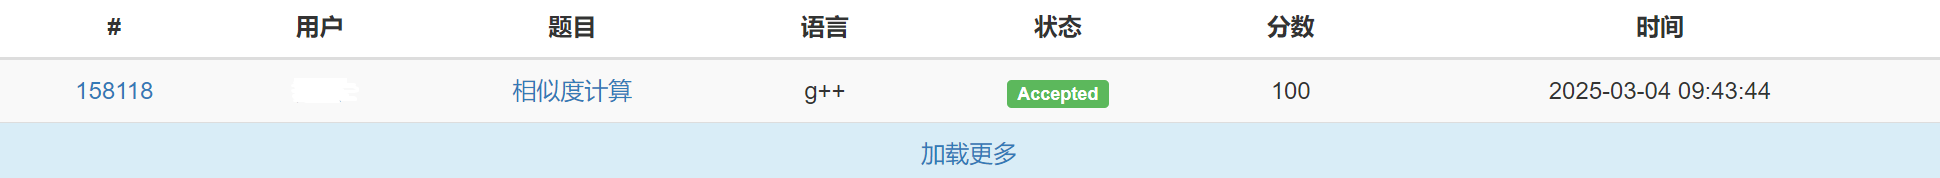
\includegraphics[width=\textwidth]{运行结果.png}
\end{figure}

}

\end{document} 